\chapter{Metodologia e Ferramentas}


\section{Sinais de Tempo Discreto e Transformada Discreta de \textit{Fourier}}

\section{Filtros Digitais}

	\subsection{Conceitos Iniciais}
	
		Os filtros digitais não contém uma implementação física em si, diferentemente dos filtros analógicos constituídos, geralmente, de associação de resistores e capacitores. Eles são construídos através de algoritmos.
		
		Para que isso possa ocorrer é necessário que o sinal de áudio (analógico) seja devidamente convertido em um sinal digital. esse sinal portanto convolui por um algoritmo de filtro adequado.
		
		De maneira geral, o projeto de um filtro consiste em obter os coeficientes para os filtros. Isso é realizado através de uma equação chamada de equação das diferenças. O processo pode ser simplesmente realizado pela equação (\ref{eq-filtro-bas}):
		
		\begin{equation}
			\text{Saida} = \sum_{1}^{n} \text{Coeficiente}_n \text{do filtro} * \text{Amostra}_n
			\label{eq-filtro-bas}
		\end{equation}
		
		Assim, o contexto de um filtro digital estará associado a equações de diferenças (ou funções de transferência no domínio Z) cujo parâmetros (coeficientes) serão calculados com o objetivo de discriminar (extrair, atenuar, etc.) determinadas componentes espectrais presentes em um sinal ou uma informação no mesmo sentido dos filtros analógicos, sem a necessidade de um circuito (\textit{hardware}) adicional. Em outras palavras, o filtro digital será uma rotina adicional agregada ao algoritmo responsável pela realização do sistema proposto em questão.
		
	\subsection{Filtros IIR}
	\label{IIR-section}	
		Os filtros digitais de resposta infinita ao impulso (\textit{Infinite Impulse Response - IIR}), também conhecidos como filtros recursivos ou autorregressivos, são modelados pela equação de diferença (\ref{eq1-iir}) ou pela função de transferência (\ref{eq2-iir-tf}), em que basicamente os valores dos coeficientes dos modelos define a natureza do filtro (passa-baixa; passa-alta; passa-faixa; rejeita-faixa).
		
		A denominação de IIR se deve que a saída do modelo decai para um valor nulo em um tempo infinito em resposta a um impulso aplicado na entrada filtro correspondente.
		
		\begin{equation}
			y(k) = \frac{1}{a_0}\left(\sum_{m=0}^{M}b_mx(k-m)-\sum_{n=1}^{N} a_ny(k-n)\right)
			\label{eq1-iir}
		\end{equation}
		
		\begin{equation}
			D(z) = \frac{y(z)}{x(z)} = \frac{b_0 + b_1z^{-1}+...+ b_mz^{-m}}{a_1z^{-1}+ a_nz^{-n}}
			\label{eq2-iir-tf}
		\end{equation}
		
		Resumidamente, a forma usual de calcular os coeficientes de um filtro digital IIR consiste em utilizar o modelo de um filtro analógico, e aplicar uma transformada Z via aproximação retangular ou trapezoidal \cite{Oppenhein1998}.
		
		Notoriamente, uma das vantagens na utilização dos filtros IIR é que eles resultam em comprimentos (quantidade de coeficientes) de filtro menor do que o filtro FIR correspondente, porém, esta melhoria é obtida às custas de distorção de fase e um transitório que não se limita a um intervalo de tempo finito \cite{Roberts1987}.
		
		Adicionalmente, conforme veremos na seção (\ref{comb-filter}) deste capítulo, um exemplo clássico de um filtro IIR é o Filtro Pente, pois se estável, a resposta simplesmente consiste em repetir 'series de impulsos que decrescem em amplitude com o tempo.
		
		
	\subsection{Filtros FIR}
		
		\begin{figure}[!htb]
			\centering
			\subfigure[\textbf{fluxo de sinais}]{
			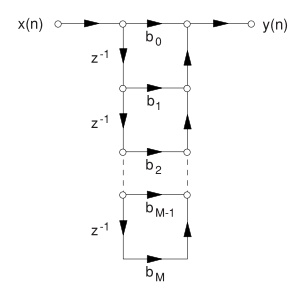
\includegraphics[scale=0.5]{./figuras/FIR-diagrama-fluxo-sinais.png}
			\label{figura1-fir}}
			\qquad
			\subfigure[\textbf{diagrama de blocos}]{
			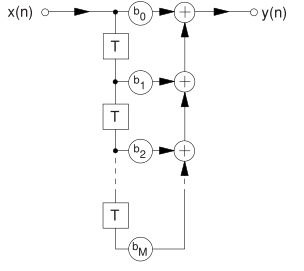
\includegraphics[scale=0.5]{./figuras/FIR-diagrama-blocos.png}
			\label{figura2-fir}}
			\caption{Diagrama de fluxo de sinais e diagrama de blocos de um filtro FIR}
			\label{fig01}	
		\end{figure}
		
		O lóbulo principal da janela retangular tem aproximadamente a metade da largura do lóbulo principal da janela \textit{Hamming};
		
		Os lóbulos laterais da janela \textit{Hamming}, em relação ao lóbulo principal, são muitos reduzidos em comparação com os da janela retangular. Especificamente, o pico de amplitude do primeiro lóbulo lateral da janela retangular está somente aproximadamente 13 dB abaixo do pico do lóbulo principal, ao passo que o valor correspondente para a janela \textit{Hamming} é de aproximadamente 40 dB.
		
		É devido a esta último ponto que a janela \textit{Hamming} reduz as oscilações na resposta em frequência de um filtro digital FIR. Todavia, há um preço a ser pago por esta melhoria, a saber, uma faixa de transição mais larga no espectro do filtro.\cite{haykin2001sinais}
	
		Vantagens:
		\begin{itemize}
			\item Um filtro não recursivo como o filtro FIR é inerentemente estável. Conforme pode ser visto na função de transferência ela é especificada em termos do zeros apenas no plano-z. Logo não há grandes preocupações em termos da escolha dos coeficientes que possam causar instabilidade no sistema, posto que seu LGR encontra-se estritamente dentro do semi-plano esquerdo do domínio-z.
			\item O filtro FIR (resposta ao impulso) tem forma simétrica no seu espectro de frequência. Isso produz uma característica de fase linear ideal, ou seja, é equivalente a puramente um atraso temporal em todas as componentes de frequência passando pelo filtro. Em outras palavras, podemos dizer que o filtro FIR não tem \textit{distorção de fase} \cite{Lynn1998}.
		\end{itemize}
	
	\subsection{Filtros Adaptativos}
	
		Os filtros adaptativos são constituídos, geralmente, por estruturas FIR, em que os coeficientes dos modelos associados são modificados conforme um procedimento adaptativo. essa modalidade de filtro geralmente é empregada nos seguintes contextos (\textit{lista não exaustiva}):
		
		\begin{itemize}
			\item Como procedimento alternativo na obtenção de valores dos coeficientes de um determinado filtro FIR, em que padrões de entrada e saída conhecidos são utilizados para estabelecer os valores dos coeficientes do filtro em questão;
			\item Cancelamento ou redução de ecos/barulhos de um determinado ambiente;
			\item Na modelagem de sistemas dinâmicos; e
			\item Como modelagem básica de representações de redes neurais artificiais.
		\end{itemize}
	
		A equação () representa o modelo de um filtro FIR, em que $W_m(k)$ denota os valores dos coeficientes do filtro em um instante de tempo $k$. 
		
		\begin{equation}
			\label{eq1-filtroadap}
			y(k) = \sum_{m=0}^{M} W_m(k)x(k-m)
		\end{equation}
		
		A diferença ou erro $\epsilon(k)$ entre o valor de padrão desejado d(k) para a a resposta do filtro e a informação da saída atual $y(k)$ do modelo associado é expressa por:
		
		\begin{equation}
			\label{eq2-filtroadap}
			\epsilon(k) = d(k)- y(k)
		\end{equation}
		
		Basicamente para ajustar os valores dos coeficientes de um filtro adaptativo tipicamente utiliza o método do gradiente para essa finalidade (fonte....), sendo o critério da somatória do erro quadrático de $\epsilon_(k)$ frequentemente utilizado na etapa de adaptação.
		
		Vale salientar, que alguns sistemas de comunicação de voz utilizam filtros adaptativos com o objetivo de cancelar ou reduzir ecos ou barulhos do ambiente. Nesse contexto, foi pensado inicialmente a utilização desse modelo de filtro para o projeto. No entanto, será explicado mais a frente a não adoção desse modelo, bem como pela utilização de um filtro FIR típico.
		
	\subsection{Filtro Pente - \textit{Comb Filter}}
	\label{comb-filter}
		
		Em termos práticos \textit{comb filter} ou “filtro pente” é uma versão atrasada do mesmo sinal, causando uma  interferência construtiva ou destrutiva de dois sons tocados simultaneamente, porém com atraso entre um para o outro. 
		
		Nesse sentido, há basicamente dois tipos de \textit{comb filters}: o (\textit{feedback comb filter}) e (\textit{feedforward comb filter}). Resumidamente, os nomes referem-se à direção em que os sinais são atrasados antes de serem adicionados à entrada. O primeiro tipo considera em adicionar a saída do filtro a entrada imediatamente posterior, enquanto o segundo considera apenas adicionar à saída do filtro as entradas presente e a mesma entrada atrasada.
		
		\begin{figure}[hbt]
			\centering
			\subfigure[\textbf{Feedback comb-filter}]{
				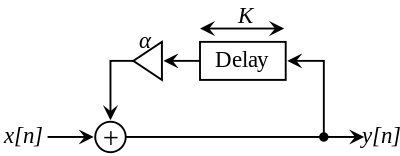
\includegraphics[scale=0.5]{./figuras/Comb_filter_feedback.png}
				\label{fig01a-combfilter}
				}
			\qquad
			\subfigure[\textbf{Feedforward comb-filter}]{
				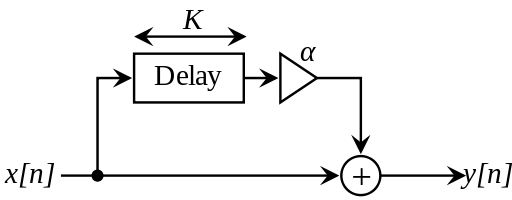
\includegraphics[scale=0.5]{./figuras/Comb_filter_feedforward.png}
				\label{fig01b-combfilter}
			}
			\caption{Filtro Pente - \textit{Comb Filter} - Formas de Realimentação}
			\label{fig01-combfilter}
		\end{figure}
		
		Como já informado, o caso do filtro pente com realimentação na saída, é um caso especial de um Filtro de Resposta Infinita (\ref{IIR-section}), posto que pode ser observado uma figura de atraso (\textit{delay}) no sentido de realimentação no sistema. Este filtro pode ser um modelo físico computacional de "séries de ecos", os quais decaem exponencialmente, bem como espaçados uniformemente no tempo \cite{JULIUSO.SMITH2010}.
		
		
		Continuando a análise do modelo do referido filtro, ve-se que a estrutura geral de um sistema de realimentação de um \textit{ feedback comb filter} pode ser mostrado através da figura \ref{fig01a-combfilter}. Além disso pode ser descrito pela seguinte equação\footnote{Para um critério de estabilidade o coeficiente $\alpha$ da equação \ref{eq01-combfilter} tem que ser menor ou igual a 1 (0db).} de diferenças \ref{eq01-combfilter}:
				
		\begin{equation}
			\label{eq01-combfilter}
			y[n] = x[n] + \alpha y[n-K]
		\end{equation}
		
		Se rearranjarmos os termos da equação para que todos as variáveis em $y$ fiquem do mesmo lado da equação e, na sequência, aplicamos a transformada Z em ambos os membros, teremos:
		
		\begin{equation}
			\label{eq02-combfilter}
			(1-\alpha z^{-K})Y(z) = X(z)
		\end{equation}
		
		Finalmente temos a função de transferência (\ref{eq03-combfilter}) correspondente ao sistema:
		
		\begin{equation}
			\label{eq03-combfilter}
			H(z) = \frac{Y(z)}{X(z)} = \frac{1}{1-\alpha z^{-K}} = \frac{z^K}{z^K-\alpha}
		\end{equation}
		
		Uma das formas de estimar a resposta de magnitude em função do valor do tempo de delay $K$ e fator de atenuação/ganho $\alpha$ é expressar $ H(z) $ em termos de módulo $|H(K,\alpha)|$, bem como, de maneira conveniente, utilizando uma substituição $ z = e^{j\omega} $.
		
		\begin{equation}
			|H(e^{j\omega})| = \frac{1}{|1-\alpha e^{-j\omega K}|},
			\qquad
			-\pi\leq \omega \leq \pi
			\label{eq04-combfilter}
		\end{equation}
		
		Nota-se pela expressão do ganho dada pela equação (\ref{eq04-combfilter}) que seu valor tem valores de resposta \textbf{periódica} indo de um valor mínimo e subindo para um valor máximo.
		
		Supondo o valor de $\alpha = 1$ ($0$ dB), para simplificar os cálculos, a amplitude da resposta reduz-se a:
		
		\begin{equation}
			\label{eq05-combfilter}
			H(w) = \frac{1}{2|sin(\omega M/2)|}
		\end{equation}

		Note ainda que para $\alpha > 0$ são produzidos picos de ressonância em:
		
		\begin{equation}
			\begin{aligned}
				\sin(\omega K/2) &= 0 \\
				\omega \frac{K}{2} &= p\pi,\quad p=0,1,2,...,K-1\\
				w_p &= 2\pi\frac{p}{K}
			\end{aligned}
		\end{equation}
		
		Ou seja, em todos harmônicos pares do filtro.
				
		Ademais, esses filtros são utilizados em toda sorte de efeitos de sons, principalmente no universos de instrumentos musicais. Vários desses filtros podem ser usados por exemplo para simular uma reverberação. (\cite{JuliusO.Smith2010})
		
		Por último, vamos falar do modelo proposto para o projeto deste trabalho, no qual consiste de uma versão mais generalista do \textit{feedback comb-filter}. Este modelo propõe a alocação de um filtro casual $H_l(z)$ na malha de realimentação, em vez de apenas um ganho de atenuação $\alpha$. A função de transferência \ref{eq02-combfilter} pode ser então reescrita como:
		
		\begin{equation}
			H(z) = \frac{1}{1-H_l(z)z^{-K}}
		\end{equation}
		
		\begin{mymdframed}{NOTA}
			Para o critério de estabilidade do sistema, a amplitude de resposta do filtro $ H_l(z) $ deverá ser menor que 1 em todas as frequências, i.e, $ |H_l(e^{j\omega T})| < 1, \forall \omega T \in [-\pi,\pi)$
		\end{mymdframed}
		
		
		
\section{Conversão Digital Analógica}

\section{Conversão Analógica Digital}

\section{Comunicação Serial I2C}
	
\section{Ferramentas Computacionais}

	\subsection{\textit{Code Compose Studio}}
	
	\subsection{\textit{WinFilter}}
